
% \begin{frame}{Echoes and Room Impulse Response}

%     \begin{columns}[onlytextwidth]
%         \begin{column}{0.60\textwidth}
%             \begin{block}{RIRs can be modeled with the Image Methods}
%                 \begin{itemize}
%                     \item \textbf{specular reflection} only
%                     \item for cuboid room, \textbf{it is} the sound prop.
%                     \item in general, \textbf{well models the early part} of RIRs.
%                     \item unique for each source and mic source
%                 \end{itemize}
%             \end{block}
%         \end{column}
%         \begin{column}{0.38\textwidth}
%             \centering
%             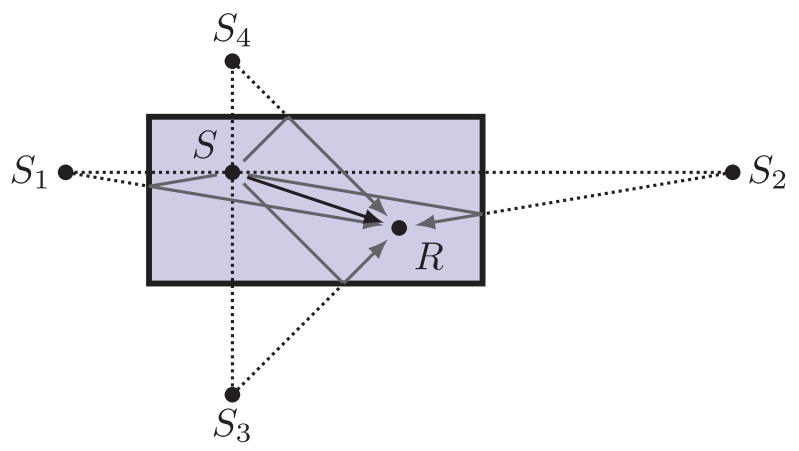
\includegraphics[width=0.8\textwidth]{figures/ism.png}
%             {\small\itshape ``playing billiard in a concert hall''}
%         \end{column}
%     \end{columns}

%     \vspace{2mm}
%     \pause
%     \begin{columns}[onlytextwidth]
%         \begin{column}{0.45\textwidth}
%             \centering
%             % \textbf{Time domain}
%             \begin{equation*}
%                 h_i^e(t) = \sum_{r=0}^{R} \alpha_i^{(r)} \delta(t - \tau_i^{(r)})
%             \end{equation*}
%             {\small sum of Dirac's delta}
%         \end{column}%
%         \pause
%         \begin{column}{0.05\textwidth}
%             \centering
%             $\overset{\text{more realistic}}{\longrightarrow}$
%         \end{column}%
%         \begin{column}{0.45\textwidth}
%             \centering
%             % \textbf{Frequency domain}
%             \begin{equation*}
%                 H_i^e(f) = \sum_{r=0}^{R} \alpha_i^{(r)}(f) \cste^{-\csti 2 \pi f \tau_i^{(r)}}
%             \end{equation*}
%             {\small sum of filters}
%         \end{column}
%     \end{columns}

%     \pause
%     \vfill
%     \begin{block}{RIRs accounts for}

%         \vspace{3mm}
%         \begin{columns}[T,onlytextwidth]
%             \column{0.48\textwidth}
%             the \textbf{geometry} of the room
%             \begin{itemize}
%                 \item \alert{Room shape and size}
%                 \item \alert{Mic and Source position}
%                 \item other objects (eg. reflectors)
%             \end{itemize}
%             \column{0.48\textwidth}
%             the \textbf{acoustic properties} of
%             \begin{itemize}
%                 \item surface materials
%                 \item objects materials
%             \end{itemize}
%         \end{columns}
%     \end{block}

%     \pause
%     \begin{mydefblock}{Echoes}
%         \centering
%         strong and distinct specular reflection
%     \end{mydefblock}

% \end{frame}

% \begin{frame}{Echoes in (Digital) Signal Processing}

%     \begin{block}{Room Impulse Response}
%         \begin{equation*}
%             \tilde{x}_i = (\tilde{h}_i \ast \tilde{s})(t) \longrightarrow \tilde{X}_i( f) = \tilde{H}_{ij}( f) \tilde{S}( f)
%         \end{equation*}
%         the linear filtering effect due to the propagation of sound from a source to a microphone in a indoor space
%     \end{block}

%     \begin{block}{Observation}
%         Our vision is limited both in time (finite and discrete) and in frequency (finite and discrete)
%         \begin{equation}
%             x_i[n] = ...
%         \end{equation}
%     \end{block}

%     \begin{block}{Signal model in the frequency domain}
%         \begin{equation*}
%             x_i = (h_i \ast s)(t)\;\longrightarrow\;X(f) = H_i(f) S(f)
%         \end{equation*}
%     \end{block}

%     \begin{block}{Approximations}
%         \begin{itemize}
%             \item Narrowband Approximation
%             \item DTFT echo model in the DFT
%         \end{itemize}
%     \end{block}

% \end{frame}

%% \subsection*{interim conclusion}
% \begin{frame}{Interim Conclusion I}
%     \begin{alertblock}{Approximations}
%         \begin{itemize}
%             \item Echoes are well described by specular reflection
%             \item Echoes are off-grid by nature
%             \item Sampling and quantization make them hard
%             \item Processing in the discrete frequency domain, but with continuous time echo model
%         \end{itemize}
%     \end{alertblock}
% \end{frame}